\chapter{講義 1：弦理論の諸問題}

\lectureoverview{還元主義への挑戦は、\(1+1\)次元におけるボソン化、電気--磁気双対性、Dブレーン、強結合転移、創発的幾何、そして弦真空の組合せ的ランドスケープを通じて鋭くなる。同じ物理系が根本的に異なる素朴な記述を持ちうる。どちらの記述が単純に見えるかは、結合定数と幾何に依存する。}

\section{還元主義、複雑性、そして単純さの問題}

サスキンドは、意図的に親しみやすい哲学的スローガンから始める。大きなものは小さなものからできており、小さなものはさらに小さなものからできている、というものである。次に彼は同じ考えのより野心的な版、基礎物理学にとって本当に重要な版を付け加える。より深い層へと降りていくにつれて、対象はより小さくなるだけでなく、より単純にもなるはずだ、というものである。彼の比喩は、家はレンガからできており、家をレンガと間違える人はいない、というものである。レンガはより小さいが、より単純でもある。

この講義の最初の一手は、その期待を素粒子物理学の実際の状況と突き合わせることである。もし還元主義がその強い意味で増大する単純さをもたらしているのなら、現在の素粒子物理学は簡素に近いはずだと期待されるかもしれない。そうではなく、サスキンドは、量子重力が入る前でさえ、帳簿付けはすでに messy に見えると強調する。講義ではこれらは粗い数え上げであるが、その粗さ自体が論点の一部である：
\begin{equation}
\begin{aligned}
N_{\mathrm{species}}&\sim 75,\\
N_{\mathrm{independent}}&\sim 10\text{--}20,\\
N_{\mathrm{parameters}}&\sim 20.
\end{aligned}
\end{equation}
話はこれで終わらない。標準模型は重力を含まず、暗黒物質を説明せず、インフレーションに必要な余分な構造を与えず、深刻な微調整問題を抱えている。通常の修復機構を加えると、数え上げは増えるだけである。超対称性が講義の例である。講義の時点で、多くの物理学者は大型ハドロン衝突型加速器が超対称パートナーを露わにすることを望んでいた。サスキンドは、対応する拡張は帳簿付けを直ちに単純化するどころか、百を超える追加パラメータを導入することになると強調する。彼の図式的なメッセージは
\begin{equation}
N_{\mathrm{parameters}}^{\mathrm{extended}} \sim 200.
\end{equation}
これらの数は意図的に粗く、歴史的なものである。それらは、より深い記述が、その粒子の目録と測定された定数のレベルで必ずしもより単純に見える必要はない、という議論に資する。

この定量的な不満は、まだサスキンドの主テーゼではない。それは前奏曲である。より深い主張、そして講義の残りを駆動する主張は、現代の量子場理論と弦理論が、レンガと家の間の一意で結合定数に依存しない区別を明らかに支持しているわけではない、というものである。次の例は、``素粒子''の意味そのものが、どの変数が効率的であるかに依存しうることを示すために選ばれている。

\section{ボソン化：固定された基礎性の最初の崩壊}

サスキンドの最初の理論的例は、\(1+1\)次元量子場理論、すなわち空間一次元、時間一次元から来る。彼はすぐに、その等価性を詳細に導出するつもりはないと宣言する。要点は形式的な証明ではなく、概念的教訓である。

フェルミオンの場の理論から始める。フェルミオン場は\(\psi\)で表される。近接する二つのフェルミオンはボソン的複合体を形成しうる。対応するボソン場は\(\phi\)で表される。一見すると階層は単純に見える。\(\psi\)が基本的であり、\(\phi\)は複合または有効変数である。講義では、ボソンはまさにこのように、フェルミオンの束縛対を生成する場として導入される。

しかし発見されたのは、同じ理論が反対の出発点から書き直せるということである。ボソン場\(\phi\)から始めてもよい。するとフェルミオンはもはや点状の構成要素として現れない。代わりに、ボソン場のキンク、すなわち\(\phi\)が二つの漸近値の間を滑らかに補間する拡張的配置として現れる。講義の最小限の数学的内容はこの漸近構造である：
\begin{equation}
\phi(x\to -\infty)=\phi_-,
\qquad
\phi(x\to +\infty)=\phi_+.
\end{equation}
便利な図式的代表は
\begin{equation}
\phi(x)\approx \frac{\phi_++\phi_-}{2}
+
\frac{\phi_+-\phi_-}{2}\tanh\!\left(\frac{x}{\ell}\right),
\end{equation}
ここで\(\ell\)は遷移領域の幅である。

\editorialnote{双曲線正接のプロファイルは、講義で描かれたキンクの標準的な滑らかな代表であり、そこで導出された式ではない。正確なボソン化の辞書は模型に依存する。概念的な要点は、フェルミオン的励起とボソン場のトポロジカルソリトンの間の交換である。}

講義で用いられたベルトの類推は、保持する価値があるほど精密である。ねじれのない平らなベルトは、キンクを持たない配位である。一端を\(2\pi\)だけ回転させると、ベルトは遠方で同じ局所的向きに戻るが、その間では広がったねじれ領域を通らなければならない。そのねじれ領域がキンクである。ボソン的記述では、フェルミオンはまさにそのような広がった対象によって表される。

結合を導入すると、この点はより鮮明になる。Susskindはこの例でそれを\(G\)と呼んでいる。主張は、二つの記述が漠然と関係しているということではなく、二つの記述の効率がパラメータ領域に依存するということである：
\begin{align}
G \ll 1
&\Rightarrow
\ell\text{ small, tight kink; }\psi\text{ efficient},\\
G \gg 1
&\Rightarrow
\ell\text{ large, broad kink; }\phi\text{ efficient}.
\end{align}
\(G\)が小さいとき、キンクは引き締まっており、フェルミオンは単純な対象のように見える。\(G\)が増大すると、キンクは広がり、フェルミオンは点状ではなくなる。そのときボソン的変数のほうがより経済的になる。

\paragraph{概略的な更新規則。}
\begin{enumerate}
\item \(\psi\)で記述されるフェルミオン的理論から始める。
\item \(\phi\)で記述されるボソン的複合体を同定する。
\item 同じ理論を完全に\(\phi\)の言葉で書き直す。
\item ボソン的記述では、フェルミオンは幅\(\ell\)のキンクとして再現する。
\item \(G\ll 1\)では、\(\ell\)は小さく、フェルミオン的記述が最も単純である。
\item より大きな\(G\)では、\(\ell\)が成長し、ボソン的記述が最も単純になる。
\end{enumerate}

これは、固定された``家とレンガ''という描像に対する最初の明示的な反例である。講義の落ちは、複合的な対象が存在するというだけではなく、何が要素的変数とみなされるかが結合によって変わりうるということである。

\section{電荷、磁気単極子、および弱結合対強結合}

次にSusskindは、同様の話がより身近な素粒子物理学にも現れるかと問う。例は電荷対磁気単極子である。電子のような通常の荷電粒子は、この言葉では電気単極子である：電場の局在した源である。磁気単極子は棒磁石の類推によって導入される。もし棒磁石の端を、目に見えない連結棒なしに何とか単離できたなら、場の線は電荷のそれとまったく同じに見えるだろうが、電気的ではなく磁気的である。

関連する制御パラメータは微細構造定数\(\alpha\)である。講義でSusskindはそれを電荷の二乗として発見法的に扱う：
\begin{equation}
\alpha \sim e^2.
\end{equation}
また彼は粗い操作的解釈も与えている：それは電子がどれほど容易に放射するかを測るものであり、彼はその強さを、加速された電子は関連する意味でおよそ``\(1/100\)''個の光子を放射すると述べることで要約している。講義自身の粗い数値的言葉では、
\begin{equation}
\alpha \approx 10^{-2}.
\end{equation}
これは精密な規約として意図されたものではなく、電荷が弱いことを符号化する教育的な方法である。

\editorialnote{弱--強の関係には、ディラック量子化という精密な祖先がある。よく用いられる一つの規約では、電気的電荷と磁気的電荷は\(e g_m=2\pi n\)を満たす。したがって、弱い電気的結合は強い磁気的結合に対応するが、正確な数値因子や保護された質量関係は理論に依存する。}

\(\alpha\ll 1\)のとき、電子が単純な対象である。その電場は弱く、その真空偏極の雲は希薄で、ほとんど点状に見える。そのとき磁気単極子は反対である：その場は巨大で、その周囲は激しく歪み、それは広く、複雑で、重い。Susskindはこの状況をまさにこの弱--強の様式で要約している：
\begin{equation}
\begin{aligned}
\alpha \ll 1
&\Rightarrow \text{simple electron;}\\
&\phantom{\Rightarrow{}}\text{heavy, extended monopole},\\
\alpha \gg 1
&\Rightarrow \text{simple monopole;}\\
&\phantom{\Rightarrow{}}\text{heavy, structured electron}.
\end{aligned}
\end{equation}
講義は単極子の質量公式を導出しない。その必要もない。要点は定性的である。\(\alpha\)が増大すると、電子の場は強まりその構造は成長し、一方で単極子は縮み軽くなる。1をはるかに超えると、有用な記述は交換される：単極子が単純で、電子が複雑になる。

これが、先のボソン化からの教訓の場の理論版である。基本的なものと複合的なものの区別は絶対的ではない。それは結合に依存する。

\begin{classroomqa}
\audiencequestion{もし還元主義が信頼できる指針でないなら、なぜ物理学者は、系を任意に小さな断片に分割するように見える微積分に依拠するのか。\lecturetimestamp{00:21:21}}
\lecturerresponse{微積分は滑らかな変化を主張するが、理論の基本的対象を同定するものではない。量子場はあらゆる距離スケールで揺らぎ、何が要素的かを一度きりで決められる最終的な滑らかな層ではなく、終わりのない階層を生み出す。}
\end{classroomqa}

このやり取りは、階層性がフラクタルに似ているという示唆へと続く。サスキンドはその類推を受け入れ、さらにそれを鋭くする。量子場はあらゆるスケールで揺らぐため、古典的な意味で決して滑らかではない。この過剰な変動こそが量子場理論を数学的に難しくしている一因であり、通常の微積分は、素朴に滑らかな微視的場に対してではなく、繰り込み済みの量に対して用いなければならない。

\section{弦、Dブレーン、そして弱--強双対性の回帰}

講義における次の移行は、意図的に素朴である。もし弦理論が基本的な構成要素の理論であるはずなら、答えはきっと単純に違いない。構成要素とは弦である。サスキンドはその期待を率直に述べ、そして講義の次の部分をその解体に費やす。

\subsection{なぜ弦がすべてではないのか}

最初の厄介な点は、避けがたく存在するDブレーンである。D\(p\)ブレーンは、弦が端を置ける\(p\)次元の物体である。文字\(D\)はディリクレ境界条件に由来するが、その名はその役割ほど重要ではない。これらの物体は理論の一部であり、捨て去ることはできない。それらは任意の飾りではない。

最も単純な例は次のとおりである。
\begin{itemize}
\item 点状であるD0ブレーン、
\item 弦状であるD1ブレーン、すなわちD弦、
\item 通常の基本弦であるF弦。
\end{itemize}
D0ブレーンは、任意の数のF弦が端を置ける重い点状の場所である。D1ブレーンは重いケーブル状の物体であり、F弦よりもはるかに太く、単位長さあたりの質量も大きいが、同様にF弦が端を置ける場所である。弱結合では、講義はこれらの物体を等しく基本的な選択肢として提示しない。Dブレーンは、重く、構造を持ち、複合的に見える物体として導入されるが、それでも理論が我々に強いるものである。

\editorialnote{講義のこの部分で用いられる奇数ブレーン理論は、タイプIIB弦理論である。その安定なDブレーンは、D1ブレーンやD3ブレーンを含む奇数空間次元を持つ。サスキンドがこれらの名称を後回しにするのは、分類ではなく双対性のパターンが当面の主題だからである。}

\paragraph{記法。}
サスキンドは講義の異なる部分で\(G\)と\(g\)をやや緩く用いている。ここでは\(G\)はボソン化の例のために取っておかれ、一方\(g\)は弦結合定数を表す。

弦結合定数\(g\)は、公理的にではなく操作的に定義される。それは、揺らぐ弦が分裂して娘弦を形成する確率を測るパラメータである。だからこそサスキンドは、それをQEDにおける\(\alpha\)の役割に直接比較する。講義はまた、張力を単位長さあたりのエネルギーと同定するために一息つく。
\begin{equation}
T=\frac{E}{L}=\frac{M}{L}.
\end{equation}

F弦とD弦について、標準的な張力の公式は弱--強の比較を明示的にする。
\begin{equation}
T_{\mathrm{F1}}=\frac{1}{2\pi\alpha'},
\qquad
T_{\mathrm{D1}}=\frac{1}{2\pi\alpha' g_s},
\qquad
\frac{T_{\mathrm{D1}}}{T_{\mathrm{F1}}}=\frac{1}{g_s}.
\end{equation}
\editorialnote{これらの張力の公式は、講義の定性的なケーブルと糸の比較の背後にある従来の規格化を与える。それらは編集上の追加であり、講義は結合定数によるスケーリングのみを用いている。}

\subsection{F弦とD弦}

弱--強の物語は、ここで弦の言葉で繰り返される。小さな結合定数では、F弦は軽く、細く、基本物体という元々の直観的イメージに近い。D弦は太く、重く、F弦の構造に満ちている。結合定数が大きくなるにつれて、F弦はより容易に分裂し、その周りに娘弦の雲が増殖し、F弦はより重く複雑になる。同時に、D弦は今や重くなったF弦を放出することがますます難しくなるため、その周囲の構造は薄くなり、D弦はより軽く、より線状になる。したがって講義の弱--強の対応は
\begin{align}
g \ll 1
&\Rightarrow
\begin{gathered}
\text{F-string light and thin;}\\
\text{D-string heavy and structured},
\end{gathered}\\
g \sim 1
&\Rightarrow
\text{F-string and D-string comparable},\\
g \gg 1
&\Rightarrow
\begin{gathered}
\text{D-string light and thin;}\\
\text{F-string heavy and structured}.
\end{gathered}
\end{align}
サスキンドは、\(g\sim 1\)付近で二つの記述が鋭く区別されなくなる、と述べる。その点を超えると、それらは事実上役割を交換する。これは電子--磁気単極子の交換の弦理論版であり、その受け入れられた名称はS双対性である。

同じ交換は、弦が閉じてループになった後にも追跡できる。弱結合では、小さなF弦ループは軽い粒子様励起であり、対応するD弦ループは重く複雑である。強結合ではそれらの役割が逆転する。D弦ループが軽い記述となり、その結果生じる軽い閉弦励起の中には重力子が含まれる。講義はこの例を用いて、なじみ深い粒子の同一性さえも、双対性のどちら側を用いるかに依存しうると主張する。

講義はこの点をさらに一歩押し進める。理想化された理論では、結合定数は単に手で調整する数ではない。それは場のように振る舞う。模式的には、
\begin{equation}
g = g(x).
\end{equation}
したがって、空間の異なる領域は異なる双対記述を好むことがあり得る。ある領域ではF弦が軽い変数であり、別の領域ではD弦がそうである。その中間では、何も特に単純ではない。だからこそSusskindにとって、弦理論は単純な還元主義的描像を回復するものではない。それは曖昧さを先鋭化するのである。

\editorialnote{摂動弦理論では、局所的な結合定数はディラトン\(g_s(x)=e^{\Phi(x)}\)によって定まる。したがって\(g=g(x)\)と書くことは単なる類推ではない。ただし、現実的なコンパクト化は一般にそのような変動を制約するポテンシャルを生じる。}

\begin{classroomqa}
\audiencequestion{結合定数が十分に変動して、別の領域でD弦がF弦より軽くなるなら、その変化は観測可能なスペクトルに影響するだろうか。\lecturetimestamp{00:34:15}}
\lecturerresponse{はい。それが、議論されている完全に対称で数学的に制御された模型を、我々の世界と直接同一視できない理由の一つである。その教訓は、整合的な量子理論が何をなし得るかに関するものであり、自然の文字通りのスペクトルに関するものではない。}
\end{classroomqa}

\begin{classroomqa}
\audiencequestion{D2ブレーンにも類似の双対記述があるだろうか。\lecturetimestamp{00:34:39}}
\lecturerresponse{はい、しかしそれは別のD弦的な交換ではない。偶数ブレーンの場合は膜解釈と追加の空間次元へと導く。それが次の構成である。}
\end{classroomqa}

\begin{classroomqa}
\audiencequestion{弦が分裂する確率が大きいことが、内部複雑性の増大を説明するのだろうか。\lecturetimestamp{00:34:53}}
\lecturerresponse{はい。機構を具体的にするためにQEDに戻ろう。電子は光子を放出し、光子は荷電対へと揺らぎ、それらの荷電線は再び放射する。結合定数を大きくすると、その階層はより希薄でなくなる。}
\end{classroomqa}

\subsection{問いに駆動された量子電磁力学への回帰}

次に学生が、分裂確率が大きいことは単により複雑な構造が``上流に''あるということを意味するだけなのかと尋ねる。Susskindは量子電磁力学に戻り、再び電子の世界線を描くことで答える。この回帰は重要である。それは、弦の話が孤立した珍奇さではなく、同じ弱--強のパターンのもう一つの実例であることを示すからである。

\begin{figure}[htbp]
\centering
\begin{tikzpicture}[scale=1.0]
\draw[->] (-1.2,0) -- (3.7,0) node[right] {space};
\draw[->] (0,-0.2) -- (0,4.3) node[above] {time};

\draw[line width=0.9pt] (0,0.2) -- (0,4.0);
\node[left] at (0,3.55) {\(e^{-}\)};

\draw[line width=0.8pt] (0,1.0) -- (0.18,1.08) -- (0.36,0.92) -- (0.54,1.10) -- (0.72,0.94) -- (0.90,1.12) -- (1.08,0.96) -- (1.26,1.14);
\draw[line width=0.8pt] (0,2.35) -- (-0.18,2.43) -- (-0.36,2.27) -- (-0.54,2.45) -- (-0.72,2.29) -- (-0.90,2.47);

\draw[line width=0.8pt] (1.26,1.14) -- (1.48,1.42);
\draw[line width=0.8pt] (1.26,1.14) -- (1.04,1.42);
\draw[line width=0.8pt] (1.48,1.42) -- (1.58,2.10);
\draw[line width=0.8pt] (1.04,1.42) -- (0.94,2.10);
\draw[line width=0.8pt] (0.94,2.10) -- (1.58,2.10);

\draw[line width=0.7pt] (1.58,1.78) -- (1.72,1.84) -- (1.86,1.72) -- (2.00,1.86);
\draw[line width=0.7pt] (0.94,1.78) -- (0.80,1.84) -- (0.66,1.72) -- (0.52,1.86);

\node at (2.35,1.95) {\(\gamma\)};
\node at (-1.15,2.75) {\(\gamma\)};
\end{tikzpicture}
\caption{講義で用いられた模式的なQED階層：点状電子が光子を放出し、光子が対を生成し、娘の荷電線が再び放射し、次第に短いスケールで構造を生じる。}
\end{figure}

講義の要点は、点状電子でさえ過程の階層を伴うということである：
\begin{enumerate}
\item 電子は光子を放出し吸収する、
\item 光子は電子--陽電子対を生成し得る、
\item 娘の荷電線自身が光子を放出し得る、
\item 階層はより小さなスケールへと続く。
\end{enumerate}
弱結合ではこの雲は希薄であり、したがって電子は実験室ではほとんど点状に見える。より強い結合ではそれは増殖し、電子は構造を持つ対象となる。弦の話は、このことの直接の類似として提示される。

同じ後半の議論は、Susskindのヒューリスティックなエネルギー計算の動機にもなっている。彼は、関係するエネルギーが単に自由粒子の寄与の和ではないと主張する。相互作用エネルギーも含めなければならない：
\begin{equation}
E_{\mathrm{tot}} = E_e + E_\gamma + E_{\mathrm{int}}.
\end{equation}
ここで\(E_{\mathrm{int}}\)が決定的な項である。これによって、着衣電子の質量が、その周囲の場と仮想構造に伴うエネルギーを含むことができる。講義はこれを形式的な繰り込み自己エネルギーの導出にはしない。要点はヒューリスティックだが本質的である：対象の質量は、その周りの複雑な雲を支えるのに必要な相互作用エネルギーをすでに含んでいる。

\begin{classroomqa}
\audiencequestion{電子が実対を生成するのに十分な自由エネルギーを含まないなら、仮想光子と電子--陽電子対のエネルギーはどこから来るのか。\lecturetimestamp{00:37:01}}
\lecturerresponse{裸の電子から始めて後からそのクーロン場を付けるということは決してない。観測される電子は着衣状態であり、その質量はすでに場と相互作用のエネルギーを含んでいる。QEDでは全エネルギーは自由電子のエネルギーと自由光子のエネルギーのみの和ではない。相互作用項が不可欠である。中間の対を仮想と呼ぶのは有用だが、エネルギーの計算は完全な相互作用状態に属する。}
\end{classroomqa}

\begin{classroomqa}
\audiencequestion{高エネルギーの探針がこの構造を明らかにするとき、探針はすでに存在していた何かを発見したのではなく、それを創り出したのだろうか？\lecturetimestamp{00:38:59}}
\lecturerresponse{その解釈上の区別は議論の余地がある。操作上は、十分に高エネルギーの散乱は計算可能で非自明な終状態を持つ。弱結合ではほとんどの事象は依然として単純に見えるが、およそ\(\alpha\)程度の割合で追加の放射や対が現れる。}
\end{classroomqa}

\begin{classroomqa}
\audiencequestion{D1ブレーンがF弦よりも重いと言われるとき、その張力もまた大きいのか？\lecturetimestamp{00:39:37}}
\lecturerresponse{はい。拡がった弦にとって、ここでの``質量''とは単位長さあたりのエネルギーを意味し、それはまさに張力である。}
\end{classroomqa}

\begin{figure}[htbp]
\centering
\includegraphics[width=0.72\textwidth]{lecture_01_figure_02.png}
\lectureframe{00:38:22.500}

\vspace{1em}

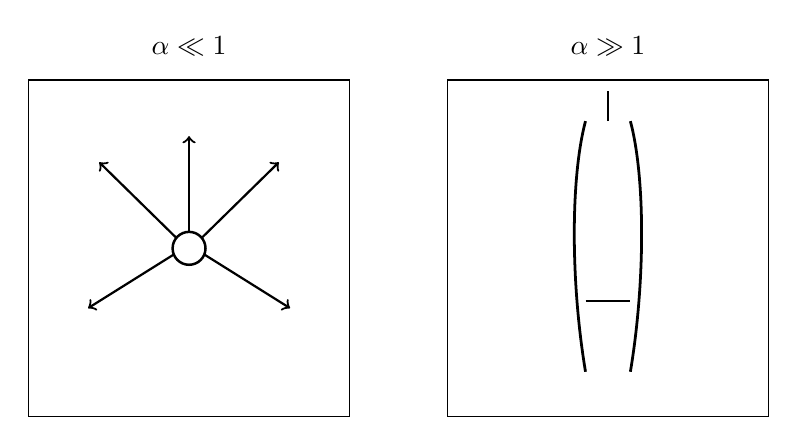
\begin{tikzpicture}[scale=0.95]
\draw (-5.3,-2.4) rectangle (-1.0,2.1);
\draw (0.3,-2.4) rectangle (4.6,2.1);

\node at (-3.15,2.55) {$\alpha \ll 1$};
\node at (2.45,2.55) {$\alpha \gg 1$};

\draw[line width=0.9pt] (-3.15,-0.15) circle (0.22);
\draw[->,line width=0.8pt] (-3.15,0.07) -- (-3.15,1.35);
\draw[->,line width=0.8pt] (-2.98,-0.01) -- (-1.95,1.00);
\draw[->,line width=0.8pt] (-3.32,-0.01) -- (-4.35,1.00);
\draw[->,line width=0.8pt] (-2.95,-0.23) -- (-1.80,-0.95);
\draw[->,line width=0.8pt] (-3.35,-0.23) -- (-4.50,-0.95);

\draw[line width=1.0pt] (2.15,-1.8) .. controls (1.95,-0.6) and (1.95,0.8) .. (2.15,1.55);
\draw[line width=1.0pt] (2.75,-1.8) .. controls (2.95,-0.6) and (2.95,0.8) .. (2.75,1.55);
\draw[line width=0.8pt] (2.15,-0.85) -- (2.75,-0.85);
\draw[line width=0.8pt] (2.45,1.55) -- (2.45,1.95);
\end{tikzpicture}
\caption{相互作用エネルギーの議論における弱--強QEDの比較。この図はSusskindの周辺で見える二つの領域、すなわち希薄な弱結合の雲と増殖する強結合の雲を分離して示している。}
\end{figure}

弱--強の比較は以前に導入されたにもかかわらず、この図がここに属する理由は、講義においてSusskindが相互作用エネルギーと増殖する構造を議論しながら、この後の質問に駆動された時点で対比を描き直すからである。

\section{偶数ブレーン理論と創発する余剰次元}

ここまで、講義は交換について強い物語を語ってきた。フェルミオン対ボソン、電子対モノポール、F弦対D弦である。次の段階はより驚くべきものである。Susskindは弦理論の別のバージョンへと切り替える。奇数次元のDブレーンではなく、偶数次元のDブレーンを持つものである。この区別が重要であるのは、この理論にはF弦と交換すべきD弦が存在しないからである。D0ブレーン、D2ブレーン、D4ブレーンなどがある。

したがって強結合極限は、単にある弦を別の弦としてラベル付けし直すことではありえない。講義によれば、もっと奇妙なことが起こる。余分な空間次元が顕在化するのである。Susskindは意図的にこれを最も劇的な形でまず述べる--- ``新しい次元が実体化する'' ---、そして直ちにより慎重な表現に翻訳する。非常に小さなコンパクトな方向が膨張し、もはや無視できなくなるのである。

帳簿付けは論点の一部であるため、彼はそこで間を置く。
\begin{equation}
\begin{aligned}
10\text{-dimensional string theory} &= 9\text{ space}+1\text{ time},\\
11\text{-dimensional theory} &= 10\text{ space}+1\text{ time}.
\end{aligned}
\end{equation}
講義の主張は、偶数ブレーン理論の強結合極限が事実上11次元であるというものである。

\editorialnote{偶数ブレーン理論はType IIA弦理論であり、その強結合完備化はM理論である。標準的な単位では、創発する円の半径と11次元プランク長は\(R_{11}=g_s\ell_s\)および\(\ell_{11}=g_s^{1/3}\ell_s\)のようにスケールする。これらの名称と公式は、講義の幾何学的な説明の背後にある現代的な辞書を明示している。}

\subsection{ピーナッツバターサンドイッチ}

コンパクトな方向を思い描くために、Susskindは``ピーナッツバターサンドイッチ''模型を用いる。無限に薄い二枚のパンがあり、その間に実空間が存在する。特別な規則は、一方の側から出ると他方の側に戻るというものである。講義が形式的ではなく絵的に説明する従来の記法では、次のように書ける。
\begin{equation}
y \sim y + 2\pi R.
\end{equation}
もし\(R\)が非常に小さければ、サンドイッチの中に住む観測者は自分の世界を事実上低次元として記述する。そのとき鍵となる強結合の更新は
\begin{equation}
g\uparrow
\qquad \Longrightarrow \qquad
R_{\mathrm{compact}}\uparrow.
\end{equation}
である。これが、Susskindが空間の新しい次元が現れると言うときに意味することである。すなわち、空間が無から創られるのではなく、以前は小さかったコンパクトな方向が膨張し、有効理論において可視的になるのである。

\begin{figure}[htbp]
\centering
\resizebox{\linewidth}{!}{%
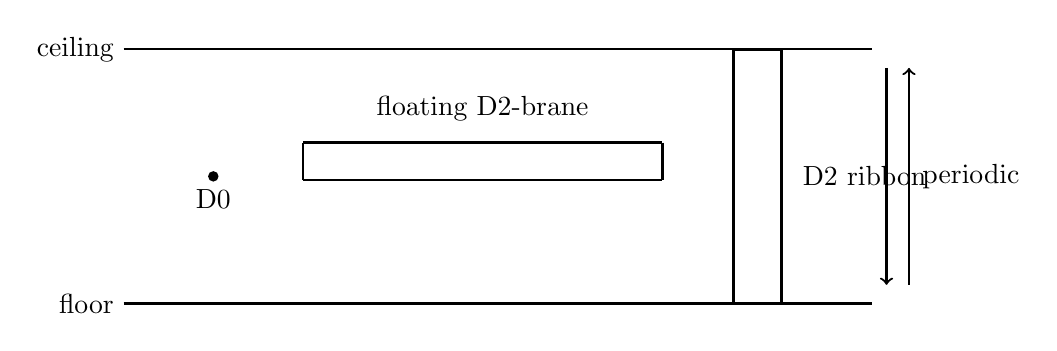
\begin{tikzpicture}[scale=0.95]
\draw[line width=0.9pt] (-5,1.7) -- (5,1.7);
\draw[line width=0.9pt] (-5,-1.7) -- (5,-1.7);

\node[left] at (-5,1.7) {ceiling};
\node[left] at (-5,-1.7) {floor};

\draw[->,line width=0.8pt] (5.2,1.45) -- (5.2,-1.45);
\draw[->,line width=0.8pt] (5.5,-1.45) -- (5.5,1.45);
\node[right] at (5.55,0) {periodic};

\draw[line width=1.0pt] (-2.6,0.45) -- (2.2,0.45);
\draw[line width=1.0pt] (-2.6,-0.05) -- (2.2,-0.05);
\draw[line width=1.0pt] (-2.6,0.45) -- (-2.6,-0.05);
\draw[line width=1.0pt] (2.2,0.45) -- (2.2,-0.05);
\node at (-0.2,0.9) {floating D2-brane};

\draw[line width=1.0pt] (3.15,-1.7) -- (3.8,-1.7);
\draw[line width=1.0pt] (3.15,1.7) -- (3.8,1.7);
\draw[line width=1.0pt] (3.15,-1.7) -- (3.15,1.7);
\draw[line width=1.0pt] (3.8,-1.7) -- (3.8,1.7);
\node[right] at (3.95,0) {D2 ribbon};

\fill (-3.8,0) circle (0.07);
\node[below] at (-3.8,-0.05) {D0};
\end{tikzpicture}
}%
\caption{サンドイッチコンパクト化。上下の境界は周期的に同一視され、一つのD2ブレーンは絨毯のようにそれらの間を浮かび、別のものは床から天井まで伸び、コンパクトな方向が小さいときには弦のように見える。}
\end{figure}

\subsection{D0ブレーンとD2ブレーンはどうなるのか？}

講義は今、D0ブレーンと弦がどうなるかを問う。答えは非対称である。\(g\)が大きくなるにつれて、D0ブレーンはますます軽くなり、高次元の解釈では新たに顕在化した方向に運動量を持つ粒子の塔に加わる。こうして、弱結合の描像における重く複雑な物体が、強結合の描像における通常の軽い励起となる。

質量関係は次の同一視を示している：
\begin{equation}
M_{D0}(n)=\frac{n}{g_s\ell_s}
=\frac{n}{R_{11}}
=M_{\mathrm{KK}}(n).
\end{equation}
\editorialnote{SusskindはD0ブレーンを11次元理論の``重力子''と呼んでいる。より正確には、それらの束縛状態が11次元超重力多重項のKaluza--Klein運動量モードであり、その質量ゼロのセクターには重力子が含まれる。この区別は、講義における物理的な同一視を保ちつつ、文字通りの一粒子の過大評価を避けている。}

D2ブレーンは弦の運命を説明する。講義で強調される配置は二つある：
\begin{enumerate}
\item ピーナッツバターの中のカーペットのように床と天井の間に浮かぶD2ブレーン；
\item リボンのように床から天井へ張られ、可視方向に沿って伸びたD2ブレーン。
\end{enumerate}
サンドイッチが薄いとき、リボンは実効的に一次元に見える。低エネルギー観測者が弦と呼ぶのはこの物体である。コンパクト方向が開くにつれて、同じ物体は紛れもなく膜的なものになる。垂直方向により多くの物質を含むようになるため、重くなり、弦らしくなくなる。

\paragraph{移行の論理。}
\begin{enumerate}
\item 非常に薄いコンパクト方向から始めると、床から天井へのリボンは実効的に弦のように振る舞う。
\item \(g\)を増やすと、コンパクト方向が膨張する。
\item D0ブレーンは軽くなり、高次元理論におけるKaluza--Klein運動量状態として再解釈される。
\item 弦のようなD2リボンは目に見えて伸びた膜となり、重くなる。
\end{enumerate}
これが、双対性から創発的幾何学への講義の蝶番である。強結合は単にある物体を別の物体に交換するのではなく、どちらの幾何学が効率的であるかを変える。

Susskindはこれがどれほど奇妙に聞こえるかについてしばし留まる。提案された同一視の網は困難な数学的整合性関係を必要とし、そのうちのいくつかは最初に物理学者たちに予想として現れ、後に数学者たちによって確立された。彼の主張は、あらゆる現実的な弦の真空が理解されているということではなく、双対性の網そのものが異常に厳しい検証を生き延びてきたということである。

この理想化された設定で結合が場所ごとに変化するならば、効率的な幾何学もそれに伴って変化しうる。ある領域は軽い弦と重いD0ブレーンを伴うほとんど10次元に見えるかもしれず、別の領域は重い巻き付いた膜と軽いKaluza--Kleinモードを伴う11次元記述へと開くかもしれない。言語の局所的な変化は同じ双対性の網の一部である。

記録はこれらの関係の名称を一時的に``不等式''と表記している。文脈上、意図された語は\emph{双対性}である：パラメータ空間の両端の間の関係である。この訂正が重要であるのは、講義の結論がまさに、基本的構成要素の一意なリストは知られていないというものであるからだ。弦、ブレーン、粒子、高次元幾何学は互いに変換しうる；網のどの成員も絶対的に基本的でないか、あるいは何らかのより深い組織化が未知のまま残っているかのいずれかである。

\section{D3ブレーン、巻き付いた膜、そして双対性の幾何学的描像}

休憩の後、Susskindはこの主題を相互に結びついた理論とアイデアの``巨大な網''であると明示的に述べる。次の例は新たな孤立した効果ではなく、以前のものを結び合わせる橋である。

\subsection{D3ブレーンの世界体積}

最初の橋はD3ブレーンを用いる。D3ブレーンは三つの空間次元を持ち、それに閉じ込められた観測者はそれを通常の空間と容易に誤認しうる。ブレーンは曲がり揺らぐことができ、一方それに端点を持つ弦は結合し、分裂し、散乱しうる。ブレーンに沿った方向のみを見る観測者にとって、各端点は粒子のように見え、端点間の相互作用は通常の量子場理論のように見える。

\begin{figure}[htbp]
\centering
\resizebox{\linewidth}{!}{%
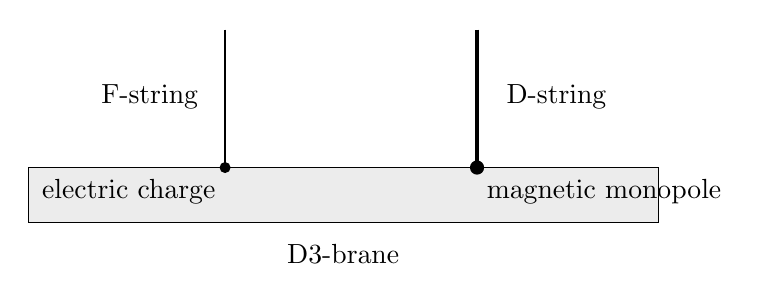
\begin{tikzpicture}[scale=1.0]
\draw[fill=gray!15] (-4,-0.35) rectangle (4,0.35);
\node at (0,-0.75) {D3-brane};

\draw[line width=0.9pt] (-1.5,2.1) -- (-1.5,0.35);
\fill (-1.5,0.35) circle (0.07);
\node[left] at (-1.72,1.25) {F-string};
\node[below left] at (-1.5,0.32) {electric charge};

\draw[line width=1.5pt] (1.7,2.1) -- (1.7,0.35);
\fill (1.7,0.35) circle (0.09);
\node[right] at (1.95,1.25) {D-string};
\node[below right] at (1.7,0.32) {magnetic monopole};
\end{tikzpicture}
}%
\caption{D3ブレーンの世界体積解釈。F弦の端点は電荷として現れ、D弦の端点は磁気単極子として現れる。}
\end{figure}

これは講義の中でも最も満足のいく同一視の一つである。D3ブレーンに端点を持つF弦は、世界体積の観測者には電荷として現れる。同じブレーンに端点を持つD弦は磁気単極子として現れる。言い換えれば、F弦とD弦の間の双対性は、D3ブレーンの世界体積上で、通常の場の理論の電磁双対性--となる。以前は類推であったものが、今や明示的な辞書となっている。

\editorialnote{D3ブレーンを重ねたものの低エネルギー世界体積上の記述は、四次元\(\mathcal N=4\)超対称Yang--Mills理論である。その電気--磁気双対性は、IIB型S双対性の場の理論における実現である。単一のブレーンは、講義で図的に用いられた可換極限を与える。}

\subsection{二つのコンパクト方向と非対称な巻き付き}

次にSusskindは高次元の幾何学に戻り、一つではなく二つの小さな方向をコンパクト化する。黒板に11次元を描くことはできないので、彼はスケッチで用いていない七つの大きな方向を一つの見える水平方向に押し込み、次に二つのコンパクトな方向を明示的に描く。彼はコンパクト化を非対称に描くことにこだわる。なぜなら、有効な弦が異なる張力をもつためには、一方のコンパクト方向が他方より短くなければならないからである。

\begin{figure}[htbp]
\centering
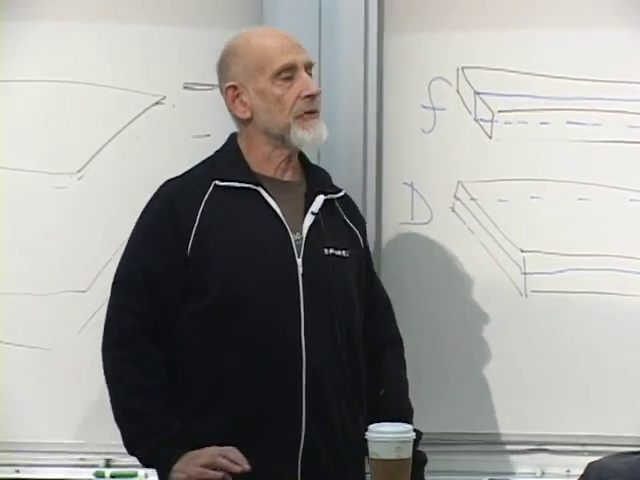
\includegraphics[width=0.78\textwidth]{lecture_01_figure_03.png}
\lectureframe{01:10:25.000}
\caption{二つの巻き付いた膜について完成した黒板の状態。短いコンパクトサイクルと長いコンパクトサイクルは、右に描かれたF弦およびD弦のようなリボンを生じる。}
\end{figure}

膜はどちらのコンパクト方向にも巻き付くことができ、非コンパクト方向から見ると弦のように見える。\(R_1\)と\(R_2\)が二つの円の半径であるなら、その有効張力は
\begin{equation}
\begin{aligned}
T_{(1)}&=2\pi R_1 T_{\mathrm{M2}},\\
T_{(2)}&=2\pi R_2 T_{\mathrm{M2}},\\
\frac{T_{(1)}}{T_{(2)}}&=\frac{R_1}{R_2}.
\end{aligned}
\end{equation}
したがって、等しくない円の大きさは等しくない弦の張力を生じる。短い方への巻き付きを軽いF弦、長い方への巻き付きを重いD弦と同定すると、概略的に
\begin{equation}
g_s\sim \frac{R_{\mathrm{short}}}{R_{\mathrm{long}}},
\qquad
\frac{T_{\mathrm{D1}}}{T_{\mathrm{F1}}}\sim \frac{1}{g_s}.
\end{equation}
と書ける。

\begin{classroomqa}
\audiencequestion{この描像における結合定数は、二つのコンパクト次元の比として理解できるか。\lecturetimestamp{01:10:13}}
\lecturerresponse{はい。弱--強パラメータはアスペクト比として幾何化される。一方の方向を短くすると小さな結合定数が生じ、二つの方向を交換すると軽い弦と重い弦が交換される。}
\end{classroomqa}

\editorialnote{講義では一時的にこの比を\(\alpha\)と呼び、以前にQEDの微細構造定数に用いた記号を再利用している。ここでは二つの意味を区別しておくために\(g_s\)と書く。完全なM理論の構成では、IIB型の結合定数はコンパクトな二次元トーラスの複素構造に符号化されており、正確な分子はそのサイクルをどのようにラベル付けするかに依存する。}

巻き付いた膜の描像は、黒板の絵の遠近の歪みなしに次のように要約できる。

\begin{figure}[htbp]
\centering
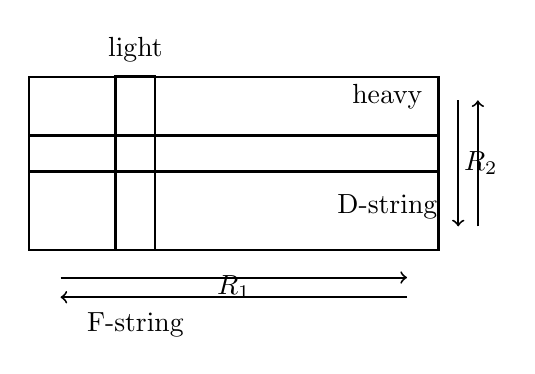
\begin{tikzpicture}[scale=1.0]
\draw[line width=0.9pt] (0,0) rectangle (5.2,2.2);
\node[below] at (2.6,-0.2) {\(R_1\)};
\node[right] at (5.4,1.1) {\(R_2\)};

\draw[->,line width=0.7pt] (5.45,1.9) -- (5.45,0.3);
\draw[->,line width=0.7pt] (5.7,0.3) -- (5.7,1.9);
\draw[->,line width=0.7pt] (0.4,-0.35) -- (4.8,-0.35);
\draw[->,line width=0.7pt] (4.8,-0.6) -- (0.4,-0.6);

\draw[line width=1.0pt] (1.1,0) -- (1.6,0) -- (1.6,2.2) -- (1.1,2.2) -- cycle;
\node at (1.35,2.55) {light};

\draw[line width=1.0pt] (0,1.45) -- (5.2,1.45);
\draw[line width=1.0pt] (0,1.00) -- (5.2,1.00);
\node at (4.55,1.95) {heavy};

\node at (1.35,-0.95) {F-string};
\node at (4.55,0.55) {D-string};
\end{tikzpicture}
\caption{二つの巻き付いた膜の配置はどちらも非コンパクト方向からは弦のように見えるが、等しくないコンパクトなスケールのために一方の有効な弦が他方より軽くなる。}
\end{figure}

これは以前の双対性の話の幾何学的な版である。一方の方向を圧縮し他方を伸ばすと、一方の巻き付いた対象が重くなり他方が軽くなるので、F弦とD弦の役割は入れ替わりうる。

\begin{classroomqa}
\audiencequestion{コンパクト方向が周期的であるなら、巻き付いた対象は無限に広いのか。\lecturetimestamp{01:10:41}}
\lecturerresponse{いいえ。コンパクトな円は、端に達することなく繰り返し周回できるとしても、有限の円周をもつ。切り開いた絵の上端と下端は同じ点を表し、ちょうど区間の端点が一つの円の点を表しうるのと同じである。}
\end{classroomqa}

\begin{figure}[htbp]
\centering
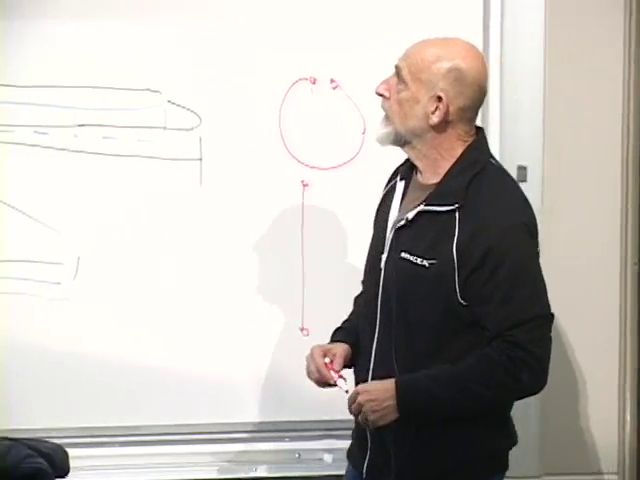
\includegraphics[width=0.78\textwidth]{lecture_01_figure_04.png}
\lectureframe{01:12:25.000}

\vspace{1em}

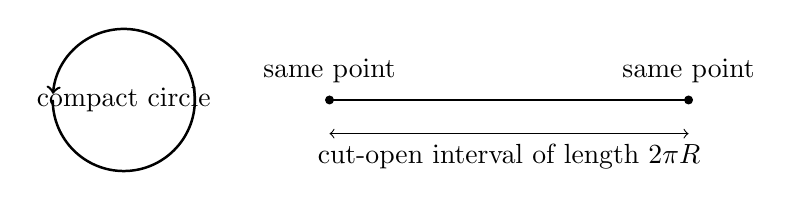
\begin{tikzpicture}[scale=0.95]
\draw[line width=0.9pt,->] (-3.7,0) arc[start angle=180,end angle=535,radius=0.95];
\node at (-2.75,0) {compact circle};
\draw[line width=0.9pt] (0.0,0) -- (4.8,0);
\fill (0.0,0) circle (0.06);
\fill (4.8,0) circle (0.06);
\draw[<->] (0.0,-0.45) -- (4.8,-0.45);
\node at (2.4,-0.75) {cut-open interval of length \(2\pi R\)};
\node[above] at (0.0,0.1) {same point};
\node[above] at (4.8,0.1) {same point};
\end{tikzpicture}
\caption{コンパクトな円とその切り開いた黒板表示。一方の端点を越えると他方で戻る。円の周りを進みながら同時に非コンパクト方向にも進むなら、代わりに螺旋を描くであろう。}
\end{figure}

\begin{classroomqa}
\audiencequestion{なぜコンパクトな経路は螺旋ではなく円なのか。\lecturetimestamp{01:12:23}}
\lecturerresponse{非コンパクト方向の各固定点において、コンパクト方向は円である。螺旋は、非コンパクト方向に進みながら同時に円の周りを巻く場合にのみ現れる。黒板上の区間は単に切り開かれた円であり、その二つの端点は同一視されている。}
\end{classroomqa}

\begin{classroomqa}
\audiencequestion{この幾何学自体が、Dブレーンが近くから調べられたときにどのようにF弦の集まりのように見えうるかを説明するのか。\lecturetimestamp{01:12:49}}
\lecturerresponse{関連は存在するが、この初等的な描像では透明ではない。それを見るにはより多くの幾何学的な道具立てが必要である。この図は双対性を整理するためのものであり、あらゆる微視的な構成要素の記述を導出するためのものではない。}
\end{classroomqa}

\begin{classroomqa}
\audiencequestion{長いコンパクト方向と短いコンパクト方向は、空間を移動するにつれて、あるいは時間が進むにつれて交換しうるか。\lecturetimestamp{01:13:35}}
\lecturerresponse{理想化された模型ではどちらも可能である。一方のサイクルを潰し他方を膨張させると、どちらの巻き付いた弦が軽いかが入れ替わる。これは``基本弦''が単なる名前であるもう一つの理由である。好ましい記述は領域ごとに、あるいは時間とともに変化しうる。}
\end{classroomqa}

\section{理想化、特別に対称な点、そしてランドスケープ}

講義の最後の楽章は、優雅な双対性の例から一歩引いて、それらが現実世界について何を語り、何を語らないのかを問う。

まず、Susskindは、精密に制御された双対性は高度に理想化された超対称理論の特徴であり、そこではボソンとフェルミオンが正確に一致した質量で現れると警告する。彼の類推はニュートン力学における円軌道である。実際の惑星運動が完全な円で尽くされるからではなく、対称で数学的に扱いやすいから、まずそれを研究するのである。まったく同じように、超対称弦理論は、自然が示すよりも対称性が高いため、解析しやすいのである。

それでもこの理想化は有益である。完全な円軌道は現実的な惑星系ではないが、より対称性の低い軌道にも生き残る特徴を表している。同様に、超対称な例は、量子力学、重力、微視的構造が整合的に共存しうる仕方を示している。Susskindの意図的に鋭い定式化によれば、扱いやすい弦理論は文字通り我々の世界の理論ではない。その価値は、より対称性が低く扱いにくい設定で再び現れそうな現象を明らかにすることにある。

\subsection{多くの結果をもたらす構成キット}

Dブレーンは利用可能な構成キットの一部にすぎない。講義ではフラックス、オービフォールド、オリエンティフォールドも挙げられている。まずコンパクトな幾何学を選び、次にどのブレーンとフラックスがそのサイクルを占めるかを選ぶ。単純なサンドイッチでさえ、浮遊するD2ブレーンを1枚、2枚、あるいは3枚挿入すると、その低次元物理を変える。そのような要素を加えたり減らしたりすると、有効な粒子、相互作用、パラメータが変化する。

講義の概略的な数え方で、6次元コンパクト空間がおよそ\(500\)個のサイクルを持ち、各サイクルが巻き付いたブレーン、フラックス、または関連する構造の\(10\)通りの選択を許すとしよう。すると構成の数は次のように増大する。
\begin{equation}
N_{\mathrm{vacua}} \sim 10^{500}.
\end{equation}
講義の数え方の論理は初等的である。
\begin{equation}
10 \times 10 \times \cdots \times 10 = 10^{500}
\end{equation}
ここで\(500\)個の因子がある。DNAの類推は同じ点をより身近な調子で述べている。
\begin{equation}
N_{\mathrm{DNA}}(500)=4^{500}.
\end{equation}
DNAの比較の際、聴衆の一人が一本の鎖に沿って4つの選択肢、A、C、G、Tがあることを確認する。この訂正は議論を変えるのではなく、むしろ補強する。局所的な選択の短いリストが何度も繰り返されることで、膨大な数の大域的配置が生じる。正確な指数が要点ではなく、Susskindは\(10^{500}\)を古い過小評価と呼んでいる。要点は組合せ論的な急増である。

これは冒頭の還元主義的期待の最終的な反転を与える。複雑な素粒子物理学は複雑な微視的規則から生じる必要はない。ちょうど複雑な生物が4つの塩基から作られた配列によって符号化されうるように、我々の真空が多くの単純な要素からなる一つの複雑な配置であるために生じうるのである。

\begin{classroomqa}
\audiencequestion{双対性で結ばれた等価な記述を同一視した後、完全な情報は、我々の世界の記述としてこれらの可能な真空のうちただ一つまたは少数だけを選び出すのだろうか。\lecturetimestamp{01:26:11}}
\lecturerresponse{おそらく制限された集合を選び出すだろうが、多くの異なる真空が到達可能なエネルギーでは極めて似て見えるかもしれない。引用されたランドスケープの数は、双対な記述を同一視した後でも依然として大きいままであり、無関係な高エネルギー的詳細は``ジャンクDNA''}のように機能しうる。\end{classroomqa}

\subsection{対称な点と一般的な複雑さ}

ランドスケープの中には特別に対称な点がある。幾何学的な描像では、等アスペクト配置
\begin{equation}
R_1=R_2,
\end{equation}
は二つの巻き付いた記述を等しく単純にする。電気--磁気の類推では、これは模式的に次で表される。
\begin{equation}
m_{\mathrm{monopole}}=m_e.
\end{equation}

\begin{figure}[htbp]
\centering
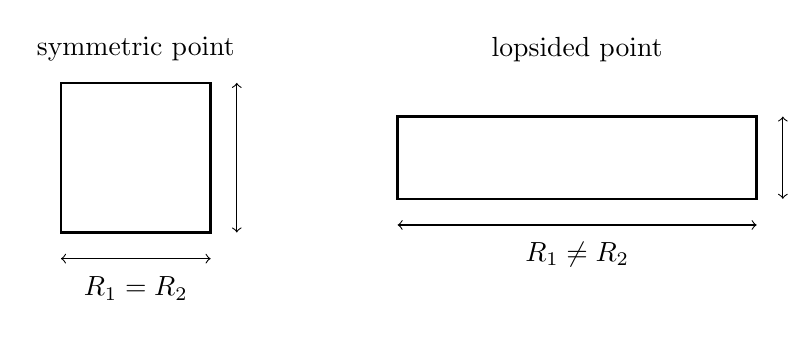
\begin{tikzpicture}[scale=0.95]
\draw[line width=0.9pt] (-4.5,-1.0) rectangle (-2.5,1.0);
\draw[<->] (-4.5,-1.35) -- (-2.5,-1.35);
\draw[<->] (-2.15,-1.0) -- (-2.15,1.0);
\node at (-3.5,1.45) {symmetric point};
\node at (-3.5,-1.75) {$R_1=R_2$};

\draw[line width=0.9pt] (0.0,-0.55) rectangle (4.8,0.55);
\draw[<->] (0.0,-0.9) -- (4.8,-0.9);
\draw[<->] (5.15,-0.55) -- (5.15,0.55);
\node at (2.4,1.45) {lopsided point};
\node at (2.4,-1.3) {$R_1\ne R_2$};
\end{tikzpicture}
\caption{等アスペクトのコンパクト化は二つの巻き付いた弦を対称に扱い、偏ったコンパクト化は一方の記述を他方よりずっと軽くする。}
\end{figure}

\begin{classroomqa}
\audiencequestion{F弦とD弦の記述が一致するために構成がずっと単純になるような真空がランドスケープの中にあるのだろうか。\lecturetimestamp{01:27:21}}
\lecturerresponse{はい、特別に対称な点はある。我々の世界はそのような点に位置しているようには見えない。身近な電気的粒子と磁気単極子は等しい質量を持たない。なぜ自然が偏った点を占めるのかは知られていない。}
\end{classroomqa}

\editorialnote{電子--モノポールの質量が等しいことは、適切に保護された自己双対模型の模式的な特徴であり、通常の超対称性のない量子電磁力学の予言ではない。これは観測された電子についての主張ではなく、講義における対称点の考え方を表している。}

サスキンドは次に、通信理論からの類推を思い起こす。ランダム符号は極めて優れたものになり得る一方、最も記述しやすく復号しやすい符号は余分な数学的構造を持ち、歴史的には性能が劣っていた。符号理論は後に非常に効果的な構造化された構成を発見したが、類推はなお残る。すなわち、簡潔に名づけられ、あるいは記述されるものは、可能なもの全体の空間の中でも非常に特別な、低複雑性の隅を占める。同様に、最も計算しやすい弦真空は、典型的でないほど単純かもしれない。

したがって、適切な問いは変わり得る。あらゆる微視的細部において厳密なコンパクト化を要求する代わりに、広いアンサンブルにわたってどの特徴が共通であるか、あるいは一般的であるかを問うことができる。サスキンドはこれを、決着した結論ではなく研究課題として提示し、計算の代わりにイデオロギー的議論を退ける。

\subsection{宇宙論的問い}

\begin{classroomqa}
\audiencequestion{巨大な円周を持つコンパクトな方向は、無限の方向と観測上異なるのか、また、我々の三つの大きな空間次元が無限であることを我々は知っているのか。\lecturetimestamp{01:30:03}}
\lecturerresponse{それらが無限であることは知られていない。閉じた三次元球面は、コンパクトでありながら膨張することができる。ほぼ平坦であることの測定は、曲率半径に関する下限を与えるにすぎない。ちょうど、ほぼ平坦な土地を測量しても、地球の表面が無限であることを証明せずに地球の大きさを制限できるのと同じである。検出された曲率または大域的識別だけが、有限のスケールを決定するであろう。}
\end{classroomqa}

\begin{classroomqa}
\audiencequestion{理想化された模型において結合が空間を通じて変動し得るなら、そのような変動は現実世界でどのように起こり得るのか。\lecturetimestamp{01:32:43}}
\lecturerresponse{対称的な例で用いられた無制限の滑らかな変動としてではない。後に論じられる現実的な可能性は、異なる有効法則を持つ領域間の離散的遷移による変動である。そのような跳びが起こるかどうかは宇宙論的問いである。}
\end{classroomqa}

\editorialnote{この応答は、あらゆる滑らかに変動するスカラー場を禁じる一般的定理としてではなく、フラックス真空と領域遷移についての講義の予告として読まれるべきである。観測は無次元結合の変動を強く制限する一方、安定化機構は、与えられた模型において連続的モジュライが利用可能なままであるかどうかを決定する。}

録音は最後の聴衆からの質問を保存していない。残っている応答は、提案された現象がある種のブラックホールについては起こり得るが、通常のシュヴァルツシルト・ブラックホールの事象の地平面では起こらない、と言っている。その地平面は、自由落下する観測者にとって局所的には普通の場所である。質問を信頼できる形で復元できないため、このやり取りにこれ以上具体的な主張は帰されない。

\section{レンガから記述の網へ}

物理学のより深い層はより単純でなければならないという希望は、もろいものと判明した。\(1+1\)次元のボソン化では、同じ理論をフェルミオンを中心に組織することも、ボソンを中心に組織することもでき、フェルミオンはキンクとして再現する。量子電気力学では、弱結合と強結合が電子と磁気単極子の記述的役割を交換する。弦理論では、F弦とD弦が同じパターンを繰り返し、偶数ブレーン理論では強結合はさらに進む。コンパクトな方向が膨張し、D0ブレーンがKaluza--Klein運動量状態となり、有効弦がより高次元の幾何学における巻き付いた膜として再解釈される。したがって、現代の量子場の理論と弦理論は、``どちらがレンガでどちらが家か''という問いに対して、唯一の最終的な答えを与えるものではない。それらは、それぞれが自らの領域で効率的である記述の網と、可能な構成の巨大な景観とを与える。その一般的な出力は単純さではなく複雑さである。
